% 'Notas de aula não oficiais de MS650 e F620' (c) 2012, 2013 de Raniere Silva
% <ra092767@ime.unicamp.br>
%
% Este trabalho é baseado nos manuscritos das notas de aula do Professor Doutor
% Jayme Vaz Júnior. para as disciplinas MS650, Métodos de Matemática Aplicada
% II, e F620, Métodos Matemáticos da Física II, disponibilizadas em
% http://www.ime.unicamp.br/~vaz/metodos2S12.htm. É permitido a este fazer uso
% deste trabalho para qualquer fim e sem nenhuma restrição.
%
% É permitido fazer uso das criações do espírito presentes neste trabalho
% diretamente relacionadas com os manuscritos das notas de aula do Professor
% Doutor Jayme Vaz Júnior única e exclusivamente para fins educacionais.
%
% Salvo indicação em contrário, este trabalho foi licenciado com a Creative
% Commons Atribuição-CompartilhaIgual 3.0 Não Adaptada. Para ver uma cópia desta
% licença, visite http://creativecommons.org/licenses/by-sa/3.0/.
%
% Este trabalho encontra-se disponível em
% https://github.com/r-gaia-cs/solucoes_ms650_f620.
%
% Este trabalho é distribuído na esperança que possa ser útil, mas SEM NENHUMA
% GARANTIA; sem uma garantia implícita de ADEQUAÇÃO a qualquer MERCADO ou
% APLICAÇÃO EM PARTICULAR.

% Este arquivo inclui o conteúdo de:
%
% * M2S12-6.pdf
% * M2S12-7.pdf

\chapter{Série de Fourier Generalizadas}
\section{O Problema de Sturm-Liouville (PSL)}
Vamos recordar alguns fatos básicos sobre o PSL. Seja
\begin{dmath*}
  L[y] = \frac{\id{}}{\id{x}}\left[ p(x) \frac{\id{y}}{\id{x}} \right] - q(x) y.
\end{dmath*}
O PSL consiste na equação diferencial
\begin{dmath*}
  L[y] + \lambda p(x) y = 0 \condition{$a \leq x \leq b$}
\end{dmath*}
com condições apropriadas conforme o problema seja regular ou singular. Uma
solução $y$ não-trivial é dita uma auto-função e a constante $\lambda$
correspondente um auto-valor.

O PSL regular corresponde ao caso em que $p(x) > 0$, $\rho(x) > 0$, $p, p', q,
\rho$ são contínuas em $x \in [a,b]$. Nesse caso as condições adequadas são:
\begin{enumerate}
  \item para condições de contorno homogêneas:
    \begin{dmath*}
      \begin{cases}
        \alpha_1 y(a) + \beta_1 y'(a) = 0, \\
        \alpha_2 y(b) + \beta_2 y'(b) = 0.
      \end{cases}
    \end{dmath*}
  \item para condições periódicas:
    \begin{dmath*}
      \begin{cases}
        y(a) = y'(b), \\
        y'(a) = y'(b).
      \end{cases}
    \end{dmath*}
  \item $y$ e $y'$ são limitadas (para $x \to a$ ou $x \to \pm \infty$ conforme
    o caso).
\end{enumerate}

E o PSL singular corresponde as
\begin{enumerate}
  \item $p(a) = 0$ ou $p(a) = 0$ e/ou $p(b) = 0$ ou $p(b) = 0$.
  \item $-\infty < x < \infty$, $0 \leq x \leq \infty$ e $-\infty < x \leq 0$.
\end{enumerate}

\begin{teo}
  As autofunções correspondentes a diferentes autovalores de um PSL regular com
  condição de contorno homoêneas ou periódicas são ortogonais com peso $\rho(x)$
  em $[a,b]$, ou seja,
  \begin{dmath*}
    \int_a^b \rho(x) u(x) v(x) \id{x} = 0.
  \end{dmath*}
  O mesmo vale para as autofunções de quadrado integrável de um PSL singular com
  a condição que estas autofunções e suas derivadas primeiras sejam limitadas
  nos extremos.
\end{teo}
\begin{proof}
  % TODO Escrever prova.
  Ver curso de MS410.
\end{proof}
\begin{exem}
  Considere o PSL dado por
  \begin{dmath*}
    \begin{cases}
      y'' + \lambda y = 0, & -\pi < x < \pi, \\
      y(-\pi) = y(\pi), \\
      y(-\pi) = y'(\pi).
    \end{cases}
  \end{dmath*}

  Esse PSL tem autovalores $\lambda = n^2$, para $n = 0, 1, 2, \ldots$ e
  auto-funções $\left\{ 1, \cos\left( n x \right), \sin\left( n x \right)
  \right\}$. Note que temos duas autofunções para o mesmo autovalor para $n = 1,
  2, \ldots$. Logo, os autovalores não são simples no caso periódico.

  Denotando
  \begin{dgroup*}
    \begin{dmath*}
      \phi_1(x) = 1,
    \end{dmath*}
    \begin{dmath*}
       \phi_{2n}(x) = \sin\left( n x \right),
    \end{dmath*}
    \begin{dmath*}
       \phi_{2n + 1}(x) = \cos\left( n x \right)
    \end{dmath*}
  \end{dgroup*}
  para $n = 1, 2, \ldots$ temos que o auto-valor correspondente a $\phi_k(x)$ é
  \begin{dmath*}
    \lambda_k = \left( \left[ \frac{k}{2} \right] - 1 \right)^2
  \end{dmath*}
  onde $\left[ a \right]$ denota a parte inteira de $a$.

  A relação de ortogonalidade é
  \begin{dmath*}
    \int_{-\pi}^\pi \phi_n(x) \phi_m(x) \id{x} = 0,
  \end{dmath*}
  para $n \neq m$, ou seja, as autofunções são ortogonais com peso $\rho(x) =
  1$.
\end{exem}
\begin{exem}
  Considere o PSL dado por
  \begin{dmath*}
    \begin{cases}
      \left[ \left( 1 - x^2 \right) y' \right]' + \lambda y = 0, & -1 < x < 1 \\
      \lim_{x \to \pm 1} | y(x) | < \infty, \\
      \lim_{x \to \pm 1} | y'(x) | < \infty.
    \end{cases}
  \end{dmath*}

  Esse é um PSL singular cujos autovalores são $\lambda = n \left( n + 1
  \right)$ para $n = 0, 1, 2, \ldots$ e as correspondentes autofunções são os
  polinômios de Legendre $P_n(x)$ definidos por
  \begin{dmath*}
    P_n(x) = \frac{1}{2^n n!} \frac{\id{}^n}{\id{x^n}}\left( x^2 - 1 \right)^n
  \end{dmath*}
  para $n = 1, 2, \ldots$ e $P_0(x) = 1$. Logo,
  \begin{dgroup*}
    \begin{dmath*}
      P_1(x) = x,
    \end{dmath*}
    \begin{dmath*}
      P_2(x) = \left( 1/2 \right) \left( 3 x^2 - 1 \right),
    \end{dmath*}
    \begin{dmath*}
      P_3(x) = \left( 1/2 \right) \left( 5 x^3 - 3 x \right), \ldots
    \end{dmath*}
  \end{dgroup*}
\end{exem}

\section{Expansão ortogonais}
Sejam $\left\{ \phi_n(x) \right\}$ para $n = 1, 2, \ldots$ funções de quadrado
integrável com peso $\rho(x)$ em $[a,b]$,
\begin{dmath*}
  \int_a^b \rho(x) \left[ \phi_n(x) \right]^2 \id{x} < \infty
\end{dmath*}
e ortogonais (com peso $\rho(x)$) para $n \neq m$,
\begin{dmath*}
  \int_a^b \rho(x) \phi_n(x) \phi_m(x) \id{x} = 0
\end{dmath*}
para $n \neq m$.

Vamos denotar por $\langle \cdot, \cdot \rangle$ o produto escalar em $L_p^2(a,
b)$:
\begin{dmath*}
  \langle f,g \rangle = \int_a^b \rho(x) f(x) g(x) \id{x}.
\end{dmath*}

Agora vamos supor que uma função $f(x)$ pode ser escrita como o limite de uma
série uniformimente convergente de múltiplos de $\phi_n(x)$, ou seja,
\begin{dmath*}
  f(x) = \sum_{k = 1}^\infty c_n \phi_n(x).
\end{dmath*}
Com isso temos que
\begin{dmath*}
  \langle f,\phi_m \rangle = \int_a^b \rho(x) f(x) \phi_m(x) \id{x}
  = \int_a^b \left( \sum_{n = 1}^\infty c_n \phi_n(x) \right) \phi_m(x) \rho(x) \id{x}
  = \sum_{n = 1}^\infty c_n \int_a^b \phi_n(x) \phi_m(x) \rho(x) \id{x}
  = \sum_{n = 1}^\infty c_n \delta_{nm} \int_a^b \left[ \phi_m(x) \right]^2 \rho(x) \id{x}
  = c_n \int_a^b \left[ \phi_m(x) \right]^2 \rho(x) \id{x}
  = c_m \langle \phi_m, \phi_m \rangle
  = c_m \| \phi_m \|^2,
\end{dmath*}
ou seja,
\begin{dmath*}
  c_n = \frac{\langle f, \phi_n \rangle}{\| \phi_n \|^2}.
\end{dmath*}

\begin{exem}
  Para a série de Fourier temos
  \begin{dgroup*}
    \begin{dmath*}
      \left\| \phi_1(x) \right\|^2 = 2 \pi,
    \end{dmath*}
    \begin{dmath*}
      \left\| \phi_k \right\|^2 = \pi
    \end{dmath*}
  \end{dgroup*}
  para $k = 2, 3, \ldots$, e portanto
  \begin{dgroup*}
    \begin{dmath*}
      c_1 = \frac{\langle f, \phi_1 \rangle}{2\pi}
      = \frac{1}{2\pi} \int_{-\pi}^\pi f(x) \id{x}
      = \frac{a_0}{2},
    \end{dmath*}
    \begin{dmath*}
      c_{2n} = \frac{\langle f, \phi_{2n} \rangle}{\pi}
      = \frac{1}{\pi} \int_{-\pi}^\pi f(x) \sin\left( n x \right) \id{x}
      = b_n,
    \end{dmath*}
    \begin{dmath*}
      c_{2n + 1} = \frac{\langle f, \phi_{2n + 1} \rangle}{\pi}
      = \frac{1}{\pi} \int_{-\pi}^\pi f(x) \cos\left( n x \right) \id{x}
      = a_n.
    \end{dmath*}
  \end{dgroup*}
\end{exem}

Diremos que $c_n$ é o coeficiente de Fourier generalizado da série de Fourier
generalizada $f(x) = \sum_{n = 1}^\infty c_n \phi_n(x)$.

Dada uma soma
\begin{dmath*}
  s_N(x) = \sum_{n = 1}^N \gamma_n \phi_n(x),
\end{dmath*}
o desvio total quadrático $\Delta_N$
\begin{dmath*}
  \Delta_N = \left\| s_N - f \right\|^2
  = \int_a^b \rho(x) \left[ s_N(x) - f(x) \right]^2 \id{x}
\end{dmath*}
é minimizado quando $\gamma_n = c_n$, ou seja, $s_N = S_N$, que é a $N$-ésima
soma parcial da série de Fourier generalizada. De fato:
\begin{dgroup*}
  \begin{dmath*}
    \Delta_N = \langle s_N - f, s_N - f \rangle
    = \langle s_N, s_N \rangle - 2 \langle s_N, f \rangle - \langle f, f \rangle,
  \end{dmath*}
  \begin{dmath*}
    \langle s_N, s_N \rangle = \sum_{n = 1}^`N \sum_{m = 1}^N \gamma_n \gamma_m \langle \phi_n, \phi_m \rangle
    = \sum_{n = 1}^N \gamma_n^2 \| \phi_n \|^2,
  \end{dmath*}
  \begin{dmath*}
    \langle s_N, f \rangle = \sum_{n = 1}^N \gamma_n \langle \phi_n, f \rangle.
  \end{dmath*}
\end{dgroup*}
Portanto,
\begin{dmath*}
  \frac{\partial \Delta_N}{\partial \gamma_k} = 2 \gamma_k \| \phi_k \|^2 - 2
  \langle \phi_k, f \rangle = 0
\end{dmath*}
que implica em
\begin{dmath*}
  \gamma_k = \frac{\langle \phi_k, f \rangle}{\| \phi_k \|^2} = c_k.
\end{dmath*}

Como $\Delta_N \geq 0$, para $\Delta_N^{\min{}}$ temos
\begin{dmath*}
  0 \leq \Delta_N^{\min{}}
  = \sum_{n = 1}^N c_n^2 \| \phi_n \|^2 - 2 \sum_{n = 1}^N c_n \langle \phi_n, f \rangle + \| f \|^2
  = \sum_{n = 1}^N \frac{\langle \phi_n, f \rangle^2}{\| \phi_n \|^2} \| \phi_n
  \|^2 - 2 \sum_{n = 1}^\infty \frac{\langle \phi_n, f \rangle}{\| \phi_n \|^2}
  + \| f \|^2,
\end{dmath*}
ou seja,
\begin{dmath*}
  \sum_{n = 1}^N \frac{\langle \phi_n, f \rangle^2}{\left\| \phi_n \right\|^2}
  \leq \left\| f \right\|^2
\end{dmath*}
e com os argumentos conhecidos para a série de Fourier segue a desigualdade de
Bessel generalizada
\begin{dmath*}
  \sum_{n = 1}^\infty \frac{\langle \phi_n, f \rangle^2}{\| \phi_n \|^2} \leq \| f \|^2.
\end{dmath*}

Dizemos que $S_N(x)$ converge na média para $f(x)$ se
\begin{dmath*}
  \lim_{N \to \infty} \left\| S_N - f \right\|^2 = \lim_{N \to \infty} \left\| \sum_{n =
  1}^N c_n \phi_n - f \right\|^2
  = 0
\end{dmath*}
e nesse caso dizemos que $\left\{ \phi_n(x) \right\}$ é completo. Uma condição
necessária e suficiente para isso é valer a identidade de Parseval generalizada,
\begin{dmath*}
  \sum_{n = 1}^\infty \frac{\langle \phi_n, f \rangle^2}{\left\| \phi_n \right\|^2} =
  \left\| f \right\|^2,
\end{dmath*}
ou ainda
\begin{dmath*}
  \sum_{n = 1}^\infty c_n^2 \| \phi_n \|^2 = \| f \|^2.
\end{dmath*}

\section{Polinômios ortogonais}
seja $\left\{ P_n(x) \right\}$, $n = 0, 1, 2, \ldots$, uma sequência de
polinômios tais que $P_n(x)$ seja de graun $n$ e que sejam ortogonais em $[a,b]$
para $n \neq m$,
\begin{dmath*}
  \langle P_n, P_m \rangle = \int_a^b \rho(x) P_n(x) P_m(x) \id{x} = 0.
\end{dmath*}
\begin{exem}
  Vários polinômios ortogonais surgem como autofunções de PSL; alguns exemplos
  são:
  \begin{dmath*}
    \frac{\id{}}{\id{x}}\left[ p(x) \frac{\id{y}}{\id{x}} \right] - q(x) y +
    \lambda \rho(x) y = 0.
  \end{dmath*}
\end{exem}
\begin{table}[!htb]
  \centering
  \caption{Polinômios otogonais que surgem como autofunções de PSL.}
  \label{tab:pol_ort_PSL}
  \begin{tabular}{|c|c|c|c|c|c|}
    \hline
    polinômio $P_n(x)$ & $p(x)$ & $q(x)$ & $\rho(x)$ & $\lambda$ & $[a,b]$ \\ \hline
    Legendre $P_n(x)$ & $\left( 1 - x^2 \right)$ & $0$ & $1$ & $n \left( n + 1 \right)$ & $-1 \leq x \leq 1$ \\ \hline
    Chebyshev $T_n(x)$ & $\left( 1 - x^2 \right)^{1/2}$ & $0$ & $\left( 1 - x^2 \right)^{-1/2}$ & $n^2$ & $-1 \leq x \leq 1$ \\ \hline
    Hermite $H_n(x)$ & $\exp(-x^2)$ & $0$ & $\exp(-x^2)$ & $2n$ & $-\infty < x < \infty$ \\ \hline
    Laguerre $L_n(x)$ & $x \exp(-x)$ & $0$ & $\exp(-x)$ & $n$ & $0 \leq x < \infty$ \\ \hline
  \end{tabular}
\end{table}
\begin{teo}
  Uma sequência de polinômios ortogonais em um intervalo finito $a \leq x \leq
  b$ é completa.
\end{teo}
\begin{proof}
  Seja $\left\{ P_n(x) \right\}$ uma sequência de polinômios ortogonais tais que
  $P_n(x)$ é de grau $n$ e seja $p_n(x)$ um polinômio de grau $n$ arbitrário.
  Então existe $c_n$ tal que $p_n(x) - c_n P_n(x)$ seja um polinômio de grau $n
  - 1$. Da mesma forma, existe $c_{n - 1}$ tal que $\left( p_n(x) - c_n P_n(x)
  \right) - c_{n - 1} P_{n - 1}(x)$ seja um polinômio de grau $n - 2$. Dessa
  forma podemos escrever
  \begin{dmath*}
    p_n(x) = \sum_{k = 0}^n c_k P_k(x).
  \end{dmath*}
  Mas, pelo teorema da aproximação de Weierstrass
  \begin{dmath*}
    \left| f(x) - p_n(x) \right| < \epsilon
  \end{dmath*}
  para $a \leq x \leq b$. Logo,
  \begin{dmath*}
    \int_a^b \left[ f(x) - p_n(x) \right]^2 \rho(x) \id{x} < \epsilon^2 \int_a^b
    \underbrace{\rho(x)}_{>0} \id{x} < \epsilon',
  \end{dmath*}
  ou seja,
  \begin{dmath*}
    \lim_{n \to \infty} \left\| f - \sum_{k = 0}^n c_k P_k \right\| = 0,
  \end{dmath*}
  de modo que $\left\{ P_n(x) \right\}$, $n = 0, 1, 2, \ldots$ é completo.
\end{proof}

\section{Série de Fourier-Legendre}
Uma série de Fourier-Legendre é uma série da forma $f(x) = \sum_{n = 0}^\infty
c_n P_n(x)$, onde $P_n(x)$ são polinômios de Legendre, dados por $P_0(x) = 1$ e
\begin{dmath*}
  P_n(x) = \frac{1}{2^n n!} \frac{\id{}^n}{\id{x}^n}\left( x^2 - 1 \right)^n,
\end{dmath*}
$n = 1, 2, \ldots$, que é chamada fórmula de Rodrigues.
\begin{prop}
  As seguintes relações e identidades são válidas:
  \begin{enumerate}
    \item $P_(x) = (-1)^n P_n(-x)$ e $P_n(1) = 1$;
    \item $P_n'(x) = x P_{n - 1}'(x) + n P_{n - 1}(x)$ para $n \geq 1$;
    \item $n P_n(x) = n x P_{n - 1}(x) + \left( x^2 - 1 \right) P_{n - 1}'(x)$ para $n \geq 1$;
    \item $P_{n + 1}'(x) - P_{n - 1}'(x) = \left( 2 n + 1 \right) P_n(x)$ para $n \geq 1$;
    \item $\left[ \id{}\left[ (1 0 x^2) P_n'(x) \right] \right] / \id{x} + n (n + 1) P_n(x) = 0$;
    \item $(n + 1) P_{n + 1}(x) = (2n + 1) x P_n(x) - n P_{n - 1}(x)$ para $n \geq 1$;
    \item $(1 - x^2) (P_n')^2 + n^2 P_n^2 = (1 - x^2) (P_{n - 1}')^2 + n^2 P_{n - 1}^2$ para $n \geq 1$;
    \item $\left[ (1 - x^2) / n^2 \right] (P_n')^2 + P_n^2 \leq 1$ para $n \geq 1$ e $|x| \leq 1$;
    \item $| P_n(x) | \leq 1$ para $|x| \leq 1$;
    \item $\int_{-1}^1 P_n(x) P_m(x) \id{x} = \left[ 2 / \left( 2 n + 1 \right) \right] \delta_{nm}$.
  \end{enumerate}
\end{prop}
\begin{proof}
    % TODO Escrever a demonstração das identidades.
\end{proof}
\begin{exem}
  Fourier-Legendre para $f(x) = x^2$.
  \begin{dgroup*}
    \begin{dmath*}
      x^2 = \sum_{n = 0}^\infty c_n P_n(x)
      \langle x^2, P_m \rangle = \sum_{n = 0}^\infty c_n \langle P_n, P_m \rangle
      = c_m \frac{2}{2m + 1}
    \end{dmath*}
    \begin{dmath*}
      c_m = \frac{2m + 1}{2} \langle x^2, P_m \rangle
      = \frac{2m + 1}{2} \int_{-1}^1 x^2 P_m(x) \id{x}
    \end{dmath*}
    \begin{dmath*}
      \langle x^2, P_m \rangle = \langle x^2, \frac{P_{m + 1}}{m + 1} - \frac{x P_m'}{m + 1} \rangle
      = \frac{1}{m + 1} \langle x^2, P_{m + 1}' \rangle - \frac{1}{m + 1} \langle x^3, P_m' \rangle
      = \frac{1}{m + 1} \left[ \left. x^2 P_{m + 1} \right|_{-1}^1 - 2 \langle
      x, P_{m + 1} \rangle \right] - \frac{1}{m + 1} \left[ \left. x^3 P_m
      \right|_{-1}^1 - 3 \langle x^2, P_m \rangle \right]
      = \frac{1}{m + 1} \left[ \underbrace{P_{m + 1}(1)}_{1} \underbrace{P_{m + 1}(-1)}_{(-1)^{m + 1}} - 2 \langle x, P_{m + 1} \rangle \right]
      - \frac{1}{m + 1} \left[ \underbrace{P_{m + 1}(1)}_{1} + \underbrace{P_m(-1)}_{(-1)^m} - 3 \langle x^2, P_m \rangle \right]
      = \frac{1}{m + 1} \left[ 1 - (-1)^{m + 1} - 1 - (-1)^m \right] - \frac{2}{m + 1} \langle x, P_{m + 1} \rangle + \frac{3}{m + 1} \langle x^2, P_m \rangle.
    \end{dmath*}
  \end{dgroup*}
  Portanto,
  \begin{dgroup*}
    \begin{dmath*}
      \left( \frac{3}{m + 1} - 1 \right) \langle x^2, P_m \rangle = \frac{2}{m
      + 1} \langle x, P_{m + 1} \rangle
    \end{dmath*}
    \begin{dmath*}
      \left( 2 - m \right) \langle x^2, P_m \rangle = 2 \langle x, P_{m + 1}
      \rangle.
    \end{dmath*}
  \end{dgroup*}
  Mas,
  \begin{dmath*}
    P_1(x) = x \Rightarrow \left( 2 - m \right) \langle x^2, P_m \rangle = 2
    \langle P_1, P_{m + 1} \rangle
  \end{dmath*}
  e portanto
  \begin{dgroup*}
    \begin{dmath*}
      m = 0 \Rightarrow 2 \langle x^2, P_0 \rangle = 2 \langle P_1, P_1 \rangle = 4 / 3
    \end{dmath*}
    \begin{dmath*}
      m \neq 0 \Rightarrow \left( 2 - m \right) \langle x^2, P_m \rangle = 0.
    \end{dmath*}
  \end{dgroup*}
    % TODO Terminar de escrever exemplo. Falta página 83.
\end{exem}

\section{Série de Fourier-Bessel}
A equação de Bessel de ordem $\nu$ ($\nu > 0$) é
\begin{dmath*}
  x^2 y'' + x y' + \left( x^2 - \nu^2 \right) y = 0.
\end{dmath*}
Sua solução geral é da forma
\begin{dmath*}
  y = c_1 J_\nu(x) + c_2 Y_\nu(x),
\end{dmath*}
onde $J_\nu(x)$ é a função de Bessel de primeira espécie de ordem $\nu$ e
$Y_\nu(x)$ é a função de Bessel de segunda espécie de ordem $\nu$ ou função de
Neumann de ordem $\nu$. Para $J_\nu(x)$ temos
\begin{dmath*}
  J_\nu(x) = \sum_{k = 0}^\infty \frac{(-1)^k}{\Gamma(k + \nu + 1) \Gamma(k +
  1)} \left( \frac{x}{2} \right)^{2k + \nu}
\end{dmath*}
onde $\Gamma(k)$ é a função gama ($\Gamma(k + 1) = k!$ para $k \in \mathbb{N}$).

Vemos facilmente que
\begin{dgroup*}
  \begin{dmath*}
    J_0(0) = 1,
  \end{dmath*}
  \begin{dmath*}
    J_\nu(0) = 0 (\nu \neq 0).
  \end{dmath*}
\end{dgroup*}
Já para $Y_\nu(x)$ temos
\begin{dmath*}
  \lim_{x \to 0^+} Y_\nu(x) = -\infty
\end{dmath*}
devido á convergência logaritmica (termo da forma $\ln x \sum c_n x^n$).
\begin{prop}
  As seguintes identidades e relações são válidas:
  \begin{enumerate}
    \item $\left[ \id{}\left( J_\nu(x) / x^{\nu} \right) / \id{x} \right] = -
      J_{\nu + 1}(x) / x^{\nu}$ para $\nu \geq 0$;
    \item $\left[ \id{}\left( x^{\nu} J_\nu(x) \right) / \id{x} \right] =
      x^{\nu}
      J_{\nu - 1}(x)$ para $\nu \geq 1$;
    \item $J_{\nu + 1}(x) - J_{\nu - 1}(x) = - 2 J_\nu'(x)$ para $\nu \geq 1$;
    \item $J_{\nu + 1}(x) + J_{\nu + 1}(x) = \left( 2 \nu / x \right) J_\nu(x)$;
    \item $J_n(x) / x^n = \left( -x^{-1} \id{} / \id{x} \right)^n \left( J_0(x)
      \right)$ para $\nu = n \in \mathbb{R}$.
  \end{enumerate}
\end{prop}
\begin{proof}
    % TODO Escrever demonstrações da proposição da página 85.
\end{proof}

Vamos agora considerar o PSL associado com a eq. de Bessel. Primeiro, vamos
fazer a mudança de variável
\begin{dmath*}
  x = \sqrt{\lambda} t.
\end{dmath*}
Na equação de Bessel,
\begin{dmath*}
  x^2 y'' + x y' + \left( x^2 - \nu^2 \right) y = 0
\end{dmath*}
que na forma auto-adjunta é
\begin{dmath*}
  \left( x y' \right)' - \left( \nu^2 / x \right) y = x y = 0
\end{dmath*}
temos em termos da variável $t$
\begin{dmath*}
  \frac{\id{}}{\id{x}}\left( t \frac{\id{y}}{\id{t}} \right) - \frac{\nu^2}{t} y
  + \lambda t y = 0,
\end{dmath*}
onde definimos $y(t) = y(\sqrt{\lambda} t)$ e usamos $\id{} / \id{t} =
\sqrt{\lambda} \id{} / \id{x}$.

A equação acima está na forma do PSL com
\begin{dgroup*}
  \begin{dmath*}
    p(t) = t,
  \end{dmath*}
  \begin{dmath*}
    q(t) = \nu^2 / t,
  \end{dmath*}
  \begin{dmath*}
    \rho(t) = t,
  \end{dmath*}
\end{dgroup*}
ou seja, trata-se de um PSL singular para $t \to 0$.

Nesse caso, as condições apropriadas são:
\begin{itemize}
  \item $y, y'$ limitadas para $t \to 0$,
  \item $c_1 y(a) + c_2 y'(a) = 0$.
\end{itemize}

\begin{obs}
  Se $y$ e $y'$ devem ser limitadas para $t \to 0$, devemos ter $y e y'$
  limitadas para $x \to o$, o que implica que devemos descartar a função de
  Bessel de segunda espécie pois esta não é limitada.
\end{obs}

% TODO Incluir equações da página 87.

\subsection{Relação de ortogonalidade}
Para $\rho(t) = t$ e $I = [0,a]$ temos que
\begin{dmath*}
  \int_0^a t J_\nu\left( \frac{\alpha_{\nu m}}{a} t \right) J_\nu\left(
  \frac{\alpha_{\nu n}}{a} t \right) \id{t} = 0,
\end{dmath*}
para $m \neq n$.

\subsection{Normalização}
Considerando
\begin{dmath}[label={normalizacao1}]
  \fder{}{t} \left( t \fder{}{t} J_{\nu}(\sqrt{\lambda} t) \right) -
  \frac{\nu^2}{t} J_{\nu}(\sqrt{\lambda} t) + \lambda t J_{\nu}(\sqrt{\lambda}
  t) = 0
\end{dmath}
e
\begin{dmath}[label={normalizacao2}]
  \fder{}{t} \left( t \fder{}{t} J_{\nu}(\sqrt{\mu} t) \right) -
  \frac{\nu^2}{t} J_{\nu}(\sqrt{\mu} t) + \mu t J_{\nu}(\sqrt{\mu} t) = 0.
\end{dmath}
Fazendo $\eqref{normalizacao1} J_{\nu} (\sqrt{\mu} t) - \eqref{normalizacao2}
J_{\nu}(\sqrt{\lambda} t)$ temos que
\begin{dmath*}
  \fder{}{t} \left( t \fder{}{t} J_{\nu}(\sqrt{\lambda} t) \right)
  J_{\nu}(\sqrt{\mu} t) - \fder{}{t} \left( t \fder{}{t} J_{\nu}(\sqrt{\mu}
  t)\right) J_{\nu}(\sqrt{\lambda} t) + \lambda t J_{\nu}(\sqrt{\lambda} t)
  J_{\nu}(\sqrt{\mu} t) - \mu t J_{\nu}(\sqrt{\mu} t) J_{\nu}(\sqrt{\lambda} t)
  = 0
\end{dmath*}
e daí
\begin{dmath*}
  (\mu - \lambda) \int_0^a t J_{\nu}(\sqrt{\mu} t) J_{\nu}(\sqrt{\lambda} t)
  \vi{t} = \int_0^a \fder{}{t} \left( t \fder{}{t} J_{\nu}(\sqrt{\lambda} t)
  \right) J_{\nu}(\sqrt{\mu} t) \vi{t} - \int_0^a \fder{}{t} \left( t
  \fder{}{t} J_{\nu}(\sqrt{\mu} t) \right) J_{\nu}(\sqrt{\lambda} t) \vi{t}
  = \left. t \fder{}{t} \left( J_{\nu}(\sqrt{\lambda} t) \right)
  J_{\nu}(\sqrt{\mu} t) \right|_0^a - \int_0^a t \fder{}{t} \left(
  J_{\nu}(\sqrt{\lambda} t) \right) \fder{}{t} \left( J_{\nu}(\sqrt{\mu} t)
  \right) \vi{t}
  - \left. t \fder{}{t} \left( J_{\nu}(\sqrt{\mu} t) \right)
  J_{\nu}(\sqrt{\lambda} t) \right|_0^a + \int_0^a t \fder{}{t} \left(
  J_{\nu}(\sqrt{\mu} t) \right) \fder{}{t} \left( J_{\nu}(\sqrt{\lambda} t)
  \right) \vi{t}
  = \left. t \fder{}{t} \left( J_{\nu}(\sqrt{\lambda} t) \right)
  J_{\nu}(\sqrt{\mu} t) \right|_0^a
  - \left. t \fder{}{t} \left( J_{\nu}(\sqrt{\mu} t) \right)
  J_{\nu}(\sqrt{\lambda} t) \right|_0^a
  = a \sqrt{\lambda} J'_{\nu}(\sqrt{\lambda} a) J_{\nu}(\sqrt{\mu} a) - a
  \sqrt{\mu} J'_{\nu}(\sqrt{\mu} a) J_{\nu}(\sqrt{\lambda} a).
\end{dmath*}
Tomando, por exemplo, $\sqrt{\lambda} = \alpha_{\nu m} / a$, temos
$J_{\nu}(\sqrt{\lambda} a) = J_{\nu}( (\alpha_{\nu m} / a) a) = 0$. Logo:
\begin{dmath*}
  \left( \mu - \frac{\alpha_{\nu m}^2}{a^2} \right) \int_0^a t
  J_{\nu}(\sqrt{\mu} t) J_{\nu}\left( \frac{\alpha_{\nu m} t}{a} \right) \vi{t}
  = \alpha_{\nu m} J'_{\nu} (\alpha_{\nu m}) J_{\nu}(\sqrt{\mu} a).
\end{dmath*}
Note que tomando $\sqrt{\mu} = \alpha_{\nu m} / a$, temos a relação de
ortogonalidade para $n \neq m$. Derivando a expressão acima com relação a
$\sqrt{\mu}$:
\begin{dmath*}
  2 \sqrt{\mu} \int_0^a t J_{\nu}(\sqrt{\nu} t) J_{\nu}\left(
  \frac{\alpha_{\nu m} t}{a} \right) \vi{t} + \left( \mu - \frac{\alpha_{\nu
  m}^2}{a^2} \right) \int_0^a t^2 J'_{\nu}(\sqrt{\nu} t) J_{\nu} \left(
  \frac{\alpha_{\nu m} t}{a} \right) \vi{t}
  = \alpha_{\nu m} a J'_{\nu}(\alpha_{\nu m}) J'_{\nu}(\sqrt{\nu} a).
\end{dmath*}
Tomando agora $\sqrt{\nu} = \alpha_{\nu m} / a$, temos
\begin{dgroup*}
  \begin{dmath*}
    2 \frac{\alpha_{\nu m}}{a} \int_0^a t J_{\nu}^2 \left( \frac{\alpha_{\nu m}
    t}{a} \right) \vi{t} = \alpha_{\nu m} a \left[ J'_{\nu}(\alpha_{\nu m})
    \right]^2
  \end{dmath*}
  \begin{dmath*}
    \int_0^a t J_{\nu}^2\left( \frac{\alpha_{\nu m} t}{a} \right) =
    \frac{a^2}{2} \left[ J'_{\nu}(\alpha_{\nu m}) \right]^2.
  \end{dmath*}
\end{dgroup*}
Mas temos as relações:
\begin{dgroup*}
  \begin{dmath*}
    J_{\nu + 1} - J_{\nu - 1} = - 2 J'_{\nu},
  \end{dmath*}
  \begin{dmath*}
    J_{\nu - 1} + J_{\nu + 1} = (2 \nu / x) J_\nu
  \end{dmath*}
\end{dgroup*}
e portanto
\begin{dgroup*}
  \begin{dmath*}
    J_{\nu + 1} - \left( \frac{2 \nu}{x} J_{\nu} - J_{\nu + 1} \right) = -2
    J'_{\nu}
  \end{dmath*}
  \begin{dmath*}
    2 J_{\nu + 1} - \frac{2 \nu}{x} J_{\nu} = -2 J'_{\nu}
  \end{dmath*}
  \begin{dmath*}
    2 J_{\nu + 1}(\alpha_{\nu m}) - \frac{2 \nu }{\alpha_{\nu m}}
    J_{\nu}(\alpha_{\nu m}) = -2 J'_{\nu}(\alpha_{\nu m}).
  \end{dmath*}
\end{dgroup*}
Como $J_{\nu}(\alpha_{\nu m}) = 0$ então $J'_{\nu}(\alpha_{\nu m}) = -J_{\nu +
1}(\alpha_{\nu m})$ e daí
\begin{dmath*}
  \int_0^a t J_{\nu}^2\left( \frac{\alpha_{\nu m} t}{a} \right) \vi{t} =
  \frac{a^2}{2} \left[ J_{\nu + 1}(\alpha_{\nu m}) \right]^2.
\end{dmath*}
Resumindo:
\begin{dmath*}
  \int_0^a t J_\nu(\frac{\alpha_{\nu m} t}{a} J_{\nu}\left(
  \frac{\alpha_{\nu m} t}{a} \right) \vi{t} = \sigma_{mn} \frac{a^2}{2} J_{\nu +
  1}^2(\alpha_{\nu m}).
\end{dmath*}

\begin{exem}
  Obtena a expansão de $f(x) = x^{\nu}$ em série de Fourier-Bessel de ordem
  $\nu$.

  Temos que $f(x) = \sum_{n = 1}^{\infty} c_n J_{\nu} (\alpha_{\nu n} x / a)$
  implica que
  \begin{dmath*}
    \int_0^a x f(x) J_{\nu} \left( \frac{\alpha_{\nu m} x}{a} \right) \vi{x} =
    \sum_{n = 1}^{\infty} c_n \int_0^a x J_{\nu} \left( \frac{\alpha_{\nu n}
    x}{a} \right) J_{\nu}\left( \frac{\alpha_{\nu m} x}{a} \right) \vi{x}
    = \sum_{n = 1}^{\infty} c_n \frac{a^2}{2} \left[ J_{\nu + 1}(\alpha_{\nu n})
    \right]^2 \delta_{nm}
  \end{dmath*}
  e portanto
  \begin{dmath*}
    c_n = \frac{2}{a^2 \left[ J_{\nu + 1}(\alpha_{\nu n}) \right]^2} \int_0^a
    x^{\nu + a} J_{\nu}\left( \frac{\alpha_{\nu n} x}{a} \right)
    = \frac{2}{a^2 \left[ J_{\nu + 1}(\alpha_{\nu n}) \right]^2} I.
  \end{dmath*}
  Mas
  \begin{dmath*}
    \fder{}{x} \left[ x^{\nu} J_{\nu} \right] = x^{\nu} J_{\nu - 1}
  \end{dmath*}
  e portanto
  \begin{dmath*}
    I = \left( \frac{a}{\alpha_{\nu n}} \right)^{\nu + 2} \int_0^{\alpha_{\nu
    n}} \left( \frac{\alpha_{\nu n} x}{a} \right) \left( \frac{\alpha_{\nu n}
    x}{a} \right)^{\nu + 1} J_{\nu}\left( \frac{\alpha_{\nu n} x}{a} \right)
    \vi{d}
    = \left( \frac{a}{\alpha_{\nu n}} \right)^{\nu + 2} \int_0^{\alpha_{\nu n}}
    y^{\nu + 1} J_{\nu}(y) \vi{y}
    = \left( \frac{a}{\alpha_{\nu n}} \right)^{\nu + 2} \int_0^{\alpha_{\nu n}}
    \fder{}{y} \left[ y^{\nu + 1} J_{\nu + 1} \right] \vi{y}
    = \left( \frac{a}{\alpha_{\nu n}} \right)^{\nu + 2} \left. y^{\nu + 1}
    J_{\nu + 1}(y) \right|_{0}^{\alpha_{\nu n}}
    = \left( \frac{a}{\alpha_{\nu n}} \right)^{\nu + 2} \left( \alpha_{\nu n}
    \right)^{\nu + 1} J_{\nu + 1}(\alpha_{\nu n})
    = \frac{a^{\nu + 2}}{\alpha_{\nu n}} J_{\nu + 1}(\alpha_{\nu n}).
  \end{dmath*}
  E assim
  \begin{dmath*}
    c_n = \frac{2}{a^2 J_{\nu + 1}^2(\alpha_{\nu n})} \frac{a^{\nu +
    2}}{\alpha_{\nu n}} J_{\nu + 1}(\alpha_{\nu n})
    = \frac{2 a^{\nu}}{\alpha_{\nu n} J_{\nu + 1}(\alpha_{\nu n})}.
  \end{dmath*}
  Portanto,
  \begin{dmath*}
    x^{\nu} = \sum_{n = 1}^{\infty} \frac{2 a^{\nu}}{\alpha_{\nu n} J_{\nu +
    1}(\alpha_{\nu n})} J_{\nu}\left( \frac{\alpha_{\nu n} x}{a} \right)
    \condition{$0 \leq x \leq a$.}
  \end{dmath*}
\end{exem}

\section{Wavelets (``Ondaletas'')}
Vamos considerar
\begin{dmath*}
  f_n(x) = \chi_{[n, n + 1)}(x)
  = \begin{cases}
    1, & n \leq x \leq n + 1, \\
    0, & n < n, x \geq n + 1.
  \end{cases}
\end{dmath*}
Evidentemente
\begin{dgroup*}
  \begin{dmath*}
    \int_{\infty}^{+\infty} f_n(x) f_m(x) \vi{x} = 0 \condition{$m \neq n$,}
  \end{dmath*}
  \begin{dmath*}
    \int_{-\infty}^{+\infty} f_n^2(x) \vi{x} = \int_n^{n + 1} \vi{x} = 1.
  \end{dmath*}
\end{dgroup*}
Logo, $\left\{ f_n(x) \right\}$ é ortogonal mas não é completo.

\begin{exem}
  Considere $f(x) = x = \sum_{n} c_n f_n$. Então
  \begin{dmath*}
    c_n = \int_{-\infty}^{+\infty} x f_n \vi{x}
    = \int_{n}^{n + 1} x \vi{x}
    = \left. x^2 / 2 \right|_{n}^{n + 1}
    = \frac{(n + 1)^2 - n^2}{2}
    = \frac{2 n + 1}{2}.
  \end{dmath*}
  Portanto
  \begin{dmath}
    x = \sum_{n = -\infty}^{+\infty} \left( \frac{2 n + 1}{2} \right) f_n.
  \end{dmath}
  \begin{figure}[htb]
    \centering
    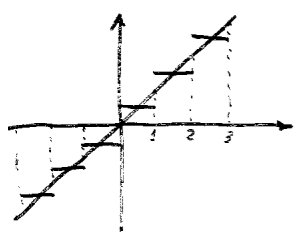
\includegraphics{figuras/07-0}
  \end{figure}
  Não é completo pois o desvio total quadrático não tende a zero quando $N \to
  \infty$.
\end{exem}

Outro conjunto:
\begin{itemize}
  \item $\phi(x) = \xi_{[0,1)}(x)$,
  \item $\phi_n(x) = \phi(x - n) = \xi_{[0,1)}(x - n) = \xi_{[n, n + 1)}(x)$.
\end{itemize}

Dilatação (binária em $2^m$) é a transformação de $\phi(x)$ em $\phi(2^m x)$.
Então
\begin{dmath*}
  \int_{-\infty}^{+\infty} \phi_(2^m x) \phi(2^m x) \vi{x} = 2^{-m}
  \int_{-\infty}^{+\infty} \phi(2^m x) \phi(2^m x) \vi{2^m x}
  = 2^{-m}.
\end{dmath*}
Pela normalização temos $2^{m / 2} \phi(2^m x)$.

Translação (diádica em $n 2^{-m}$) é a transformação de $\phi(2^m x)$ em
$\phi(2^m x - n) = \phi(2^m (x - n 2^{-m})$. Enttão
\begin{dmath*}
  \phi_{mn}(x) = 2^{m / 2} \phi(2^m x - n).
\end{dmath*}

\begin{obs}
  $\left\{ \phi_{mn} \right\}$ deve ser completo por causa da dilatação. Mas não
  é ortogonal \ldots
\end{obs}

De fato, $\phi(x)$ e $\phi(2 x)$ não são ortogonais:
\begin{dgroup*}
  \begin{dmath*}
    \phi(x) = \begin{cases}
      0, & x < 0, x \geq 1, \\
      1, & 0 \leq x < 1,
    \end{cases}
  \end{dmath*}
  \begin{dmath*}
    \phi(2x) = \begin{cases}
      0, & 2 x < 0, 2 x \geq 1, \\
      1, & 0 \leq 2 x < 1.
    \end{cases}
  \end{dmath*}
\end{dgroup*}
Então,
\begin{dmath*}
  \int_{-\infty}^{+\infty} \phi(x) \phi(2x) \vi{x} = \int_0^{1/2} 1 \cdots 1
  \vi{x}
  = 1/2
  \neq 0
\end{dmath*}
e $\phi(x)$ e $\phi(2x)$ não são ortogonais mas $\psi(x) = \phi(2x) - \phi(2x -
1)$ é.
\begin{dgroup*}
  \begin{dmath*}
    \phi(2x) = \begin{cases}
      0, & x < 0, x \geq 1/2, \\
      1, & 0 \leq x < 1/2,
    \end{cases}
  \end{dmath*}
  \begin{dmath*}
    \phi(2x - 1) = \phi(2 (x - 1/2))
    = \begin{cases}
      0, & x < 1/2, x \geq 1, \\
      1, & 1/2 \leq x < 1.
    \end{cases}
  \end{dmath*}
\end{dgroup*}
\begin{figure}[htb]
  \centering
  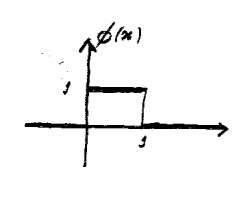
\includegraphics{figuras/07-1}
  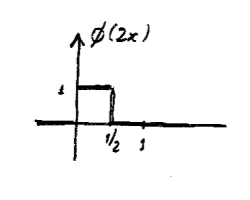
\includegraphics{figuras/07-2}
  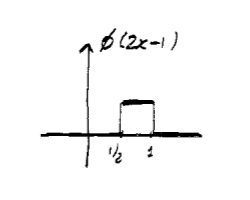
\includegraphics{figuras/07-3}\\
  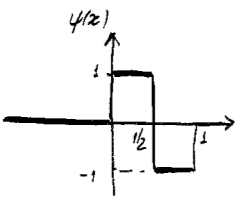
\includegraphics{figuras/07-4}
\end{figure}

Considerando $\psi_{mn}(x) = 2^{m/2} \psi(2^m x - n)$, wavelets de Haar, que é
ortogonal e completo, temos
\begin{figure}[htb]
  \centering
  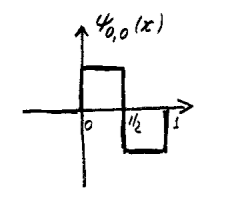
\includegraphics{figuras/07-5}
  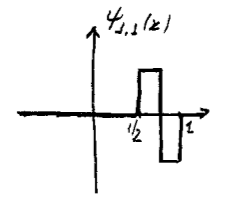
\includegraphics{figuras/07-6}
  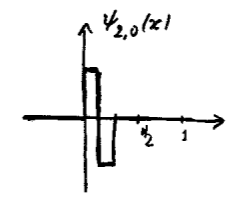
\includegraphics{figuras/07-7}
\end{figure}

Assim:
\begin{dgroup*}
  \begin{dmath*}
    f(x) = \sum_{m = -\infty}^{+\infty} \sum_{n = -\infty}^{+\infty} c_{mn}
    \psi_{mn}(x)
  \end{dmath*}
  \begin{dmath*}
    \langle \psi_{mn}, \psi_{m'n'} \rangle = \int_{-\infty}^{+\infty}
    \psi_{mn}(x) \psi_{m'n'}(x) \vi{x}
    = \sigma_{mm'} \sigma_{nn'}
  \end{dmath*}
\end{dgroup*}
e portanto
\begin{dmath*}
  c_{mn} = \langle f, \psi_{mn} \rangle
  = \int_{-\infty}^{+\infty} f(x) \psi_{mn}(x) \vi{x}
\end{dmath*}

\begin{exem}
  Expressar $f(x) = \sin(2 \pi x)$ em série de Fourier-Haar.
  \begin{dmath*}
    c_{mn} = 2^{m/2} \int_{-\infty}^{+\infty} f(x) \psi(2^m x - n) \vi{x} =
    2^{2/m} \int_{2^{-m} n}^{2^{-m} (n + 1)} f(x) \psi(2^m x - n) \vi{x}
    = 2^{m/2} \left[ \int_{2^{-m} n}^{2^{-m} (n + 1/2)} f(x) \vi{x} -
    \int_{2^{-m} (n + 1/2)}^{2^{-m}(n + 1)} f(x) \vi{x} \right]
  \end{dmath*}
  e portanto
  \begin{dmath*}
    c_{mn} = 2^{m/2} \left[ \int_{2^{-m} n}^{2^{-m}(n + 1/2)} \sin(2 \pi x)
    \vi{x} - \int_{2^{-m} (n + 1/2)}^{2^{-m} (n + 1)} \sin(2 \pi x) \vi{x}
    \right]
    = 2^{m/2} \left[ \int_{2^{-m} n}^{2^{-m} (n + 1/2)} \sin(2 \pi x) \vi{x} -
    \int_{2^{-m} (n + 1/2)}^{2^{-m} (n + 1)} \sin(2 \pi x) \vi{x}\right]
    = \frac{2^{m/2}}{2 \pi} \left[ \cos(2 \pi 2^{-m} n) - \cos(2 \pi 2^{-m} (n +
    1/2)) + \cos(2 \pi 2^{-m} (n + 1)) - \cos(2 \pi 2^{-m} (n + 1/2))\right]
    = \frac{2^{m/2}}{2 \pi} \left[ \cos(2^{-m + 1} n \pi) - 2 \cos(2^{-m + 1} (n
    + 1/2)) + \cos(2^{-m + 1} (n + 1) \pi)\right].
  \end{dmath*}
\end{exem}

\begin{obs}[``Nomenclatura'']
  \begin{itemize}
    \item $\phi(x)$ é função de escala (``scaling function'' ou ``father
      wavelet''),
    \item $\psi(x)$ é wavelet-mãe (``mother wavelet'') e
    \item $\left\{ \psi_{mn}(x) \right\}$ é base de wavelets.
  \end{itemize}
\end{obs}

\begin{obs}[Outras wavelets]
  \begin{itemize}
    \item $\psi(x) = (1 - x^2) \exp(-x^2 / 2)$ é wavelet ``chapéu mexicano'',
    \item $\psi(x) = \exp(i k_0 x) \exp(-x^2 / 2)$, para $k_0$ fixo, é wavelet
      de Morlet e
    \item $\psi(x) = \sin(\pi x / 2) \cos(3 \pi x / 2) / (\pi x / 2)$ é wavelet
      de Shannon.
  \end{itemize}
\end{obs}

\section[Sistemas Ortogonais]{Sistemas Ortogonais de Funções de Várias Variáveis}
O produto escalar é definido como
\begin{dmath*}
  \langle f, g \rangle = \iint_R \rho(x, y) f(x, y) g(x, y) \vi{x} \vi{y}.
\end{dmath*}

\begin{exem}[Fourier dupla]
  Considere
  \begin{dmath*}
    f(x, y) = \frac{a_0}{4} + \sum_{m = 1}^{\infty} \sum_{n = 1}^{\infty} \left(
    a_{mn} \cos(m x) \cos(n y) + b_{mn} \cos(m x) \sin(n y) + c_{mn} \sin(m x)
    \cos(n y) + d_{mn} \sin(m x) \sin(n y) \right),
  \end{dmath*}
  onde
  \begin{dgroup*}
    \begin{dmath*}
      a_0 = \frac{1}{\pi^2} \int_{-\pi}^{+\pi} \int_{-\pi}^{+\pi} f(x, y) \vi{x}
      \vi{y},
    \end{dmath*}
    \begin{dmath*}
      a_{mn} = \frac{1}{\pi^2} \int_{-\pi}^{+\pi} \int_{-\pi}^{+\pi} f(x, y)
      \cos(m x) \cos(n y) \vi{x} \vi{y}, \ldots
    \end{dmath*}
  \end{dgroup*}
  ou na forma complexa
  \begin{dmath*}
    f(x, y) = \sum_{m = -\infty}^{+\infty} \sum_{n = -\infty}^{+\infty} c_{mn}
    \exp(i m x) \exp(i n y)
  \end{dmath*}
  onde
  \begin{dmath*}
    c_{mn} = \frac{1}{(2 \pi)^2} \int_{-\infty}^{+\infty}
    \int_{-\infty}^{+\infty} f(x, y) \exp(-i m x) \exp(-i n y) \vi{x} \vi{y}
  \end{dmath*}
\end{exem}

\begin{exem}[Fourier em várias variáveis]
  Considere
  \begin{dgroup*}
    \begin{dmath*}
      x = \left( x_1, \ldots, x_N \right),
    \end{dmath*}
    \begin{dmath*}
      x \cdot y = \sum_{i = 1}^N x_i y_i,
    \end{dmath*}
    \begin{dmath*}
      f(x) = f(x_1, \ldots, x_N),
    \end{dmath*}
    \begin{dmath*}
      m = \left( m_1, \ldots, m_N \right),
    \end{dmath*}
    \begin{dmath*}
      f(x) = \sum_{m_1 = -\infty}^{+\infty} \ldots \sum_{m_N =
      -\infty}^{+\infty} c_{m_1 \ldots m_N} \exp(i m_1 x_1) \ldots \exp(i m_N
      x_N)
      = \sum_{m \in \mathbb{Z}} c_m \exp(i m \cdot x),
    \end{dmath*}
    onde
    \begin{dmath*}
      c_{m_1 \ldots m_N} = \frac{1}{(2 \pi)^N} \int_{-\infty}^{+\infty} \ldots
      \int_{-\infty}^{+\infty} f(x_1, \ldots, x_N) \exp(-i m_1 x_1) \ldots
      \exp(-i m_N x_N) \vi{x_1} \ldots \vi{x_N}
    \end{dmath*}
    e portanto
    \begin{dmath*}
      c_m = \frac{1}{(2 \pi)^N} \int_{\mathbb{R}^N} f(x) \exp(-i m x) \vi{x}
    \end{dmath*}
  \end{dgroup*}
\end{exem}
